\chapter{Building a Black Hole and the Near-Horizon Puzzle}

\lectureoverview{We shall build a black hole from three pieces: the causal diagram of flat spacetime, the Schwarzschild diagram, and Birkhoff's theorem for a spherical shell. The construction reveals that an event horizon is a global boundary and can begin in a region that is still locally flat. We then turn from causal geometry to entropy and Hawking temperature. A thermometer held near the horizon becomes arbitrarily hot, while a freely falling observer expects no local catastrophe. The closing argument asks what an outside experiment can actually establish without creating the disturbance it is meant to detect.}

\section{A Black Hole at the Temperature of Empty Space}

There was supposed to have been homework: build a black hole and bring it to class for show and tell. No one had one to display, but a calculation found through Wolfram supplied a gentler opening problem. What radius and mass would give a black hole a Hawking temperature near the \(3\,\mathrm{K}\) temperature of the cosmic microwave background?

\begin{classroomqa}
\audiencequestion{What was calculated on the website?\lecturetimestamp{00:00:39}}
\lecturerresponse{The radius of a black hole whose temperature is about \(3\,\mathrm{K}\). The point is not a precision calculation; it is an estimate of the physical scale.}
\end{classroomqa}

Such a hole would momentarily have the same temperature as its surroundings, but the equilibrium would be unstable. A Schwarzschild black hole has negative heat capacity. If it becomes slightly hotter than the bath, it emits, loses mass, and becomes hotter still. If it becomes slightly colder, it absorbs, gains mass, and becomes colder still.\editorialnote{This is the precise stability argument behind the deliberately loose classroom wording. A canonical heat bath cannot provide stable equilibrium for an isolated Schwarzschild black hole.}

The estimate begins with the characteristic wavelength of \(3\,\mathrm{K}\) radiation.

\begin{classroomqa}
\audiencequestion{What wavelength belongs to radiation at about three kelvin?\lecturetimestamp{00:02:03}}
\lecturerresponse{The room offered a centimeter, \(21\) centimeters, and even \(10\) meters before settling on the microwave range. The useful order-of-magnitude answer for the argument was about a centimeter, small enough for the jokes about a microwave oven and a breadbox.}
\end{classroomqa}

The typical Hawking quantum has wavelength comparable, up to numerical factors, with the Schwarzschild radius:
\begin{equation}
\lambda_{\mathrm{H}}\sim R_s,
\qquad
R_s=\frac{2GM}{c^2}.
\label{eq:l05-scale}
\end{equation}
Taking the classroom value \(\lambda_{\mathrm H}\sim1\,\mathrm{cm}\) gives \(R_s\sim1\,\mathrm{cm}\). Since a solar-mass black hole has a radius of a few kilometers and \(R_s\) is proportional to \(M\), the corresponding mass is roughly
\begin{equation}
M\sim10^{-5}M_\odot,
\label{eq:l05-rough-mass}
\end{equation}
which is planetary in scale. This is why the lecture arrives at an Earth-like estimate.

\begin{classroomqa}
\audiencequestion{Does that agree with the numerical result from Wolfram?\lecturetimestamp{00:05:53}}
\lecturerresponse{The reported result was nearer the mass of the Moon. That sounded small compared with the rough estimate, but either answer makes the intended point: the object is not something one could carry in a pocket.}
\end{classroomqa}

Keeping the constants explains the discrepancy. From
\begin{equation}
T_H=\frac{\hbar c}{4\pi k_B R_s},
\end{equation}
one finds, at \(T_H=3\,\mathrm{K}\),
\begin{equation}
R_s\simeq6.1\times10^{-5}\,\mathrm{m},
\qquad
M\simeq4.1\times10^{22}\,\mathrm{kg}.
\label{eq:l05-three-kelvin}
\end{equation}
That is of lunar rather than terrestrial mass. The microwave wavelength, the factor \(4\pi\), and the choice of which black-body wavelength to call typical account for the gap between the quick estimate and the numerical value.\editorialnote{Equation~\eqref{eq:l05-three-kelvin} restores the numerical factors omitted in the lecture's dimensional estimate. The estimate itself is retained because it is the route used in class.}

The arithmetic has served its purpose. We now want to build a black hole, mathematically and in imagination. The full field equations are too hard for the present purpose. Pictures will supply the basic facts.

\section{The First Working Part: Flat Spacetime}

Use polar coordinates centered on an observer and suppress the angles. The reduced coordinates are \((t,r)\), with \(r\geq0\). A point in this reduced diagram is not a point of four-dimensional spacetime; except at \(r=0\), it represents an entire two-sphere \(S^2\).

Radial light rays move at \(45^\circ\). An ingoing ray reaches the origin, and an outgoing ray leaves it along the other null direction. The infinite half-plane can be compressed into a finite Penrose wedge by a conformal transformation. The transformation is not unique. Its essential properties are that infinity is brought to a finite boundary and radial null directions remain at \(45^\circ\). In the language of the blackboard, we smush the diagram.

\begin{figure}[htbp]
\centering

\includegraphics[width=0.68\textwidth]{lecture_05_figure_02.png}
\caption{The upper half of compactified radial Minkowski spacetime. The vertical edge is \(r=0\), while the curve families crowd toward compactified infinity.}
\lectureframe{00:11:41.560}
\end{figure}

\begin{figure}[htbp]
\centering
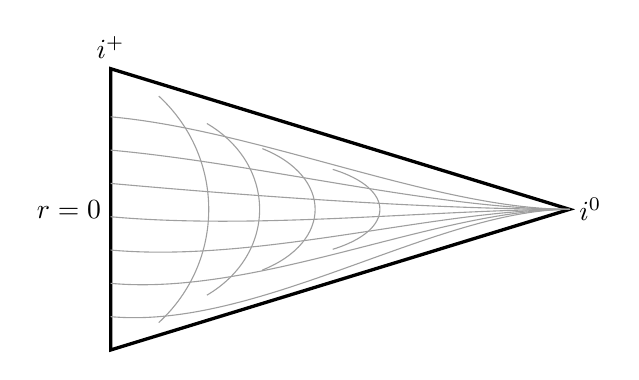
\begin{tikzpicture}[scale=0.94]
\coordinate (O) at (0,0);
\coordinate (P) at (0,3.8);
\coordinate (I) at (6.2,1.9);
\draw[very thick] (O)--(P)--(I)--cycle;
\foreach \y in {0.45,0.90,1.35,1.80,2.25,2.70,3.15} {
  \draw[gray!75] (0,\y) .. controls (2.0,\y-0.18) and (4.4,1.9) .. (I);
}
\draw[gray!75] (0.65,0.37) .. controls (1.55,1.20) and (1.55,2.60) .. (0.65,3.43);
\draw[gray!75] (1.30,0.74) .. controls (2.25,1.30) and (2.25,2.50) .. (1.30,3.06);
\draw[gray!75] (2.05,1.08) .. controls (3.00,1.46) and (3.00,2.34) .. (2.05,2.72);
\draw[gray!75] (3.00,1.36) .. controls (3.85,1.62) and (3.85,2.18) .. (3.00,2.44);
\node[left] at (0,1.9) {\(r=0\)};
\node[above] at (P) {\(i^+\)};
\node[right] at (I) {\(i^0\)};
\end{tikzpicture}
\caption{A clean version of the upper wedge. The curves are qualitative constant-\(r\) and constant-\(t\) families, not an exact coordinate grid.}
\label{fig:l05-flat-wedge}
\end{figure}

Worldlines at fixed \(r\), vertical before compactification, bow and accumulate near future timelike infinity. Constant-\(t\) slices likewise crowd toward spatial infinity. The crowding is a coordinate effect, not a physical compression of matter.

The \(45^\circ\) rule applies directly to radial light. A ray with angular momentum may miss the origin, reach a nonzero distance of closest approach, and return outward. Far from the origin its projected motion looks almost radial; only near closest approach does the reduced \((t,r)\) trajectory visibly bend. This completes the first working part.

\section{The Second Working Part: Eternal Schwarzschild}

The maximally extended Schwarzschild solution has two exterior diamonds, a future black-hole region, and a past white-hole region. Its upper and lower wavy boundaries are the future and past singularities. For a black hole made by collapse, most of this structure will soon be discarded, but the ordinary right exterior is exactly the piece we need.

\begin{figure}[htbp]
\centering

\includegraphics[width=0.72\textwidth]{lecture_05_figure_03.png}
\caption{The eternal Schwarzschild diagram, with the ordinary exterior and its schematic coordinate grid on the right.}
\lectureframe{00:16:55.975}
\end{figure}

\begin{figure}[htbp]
\centering
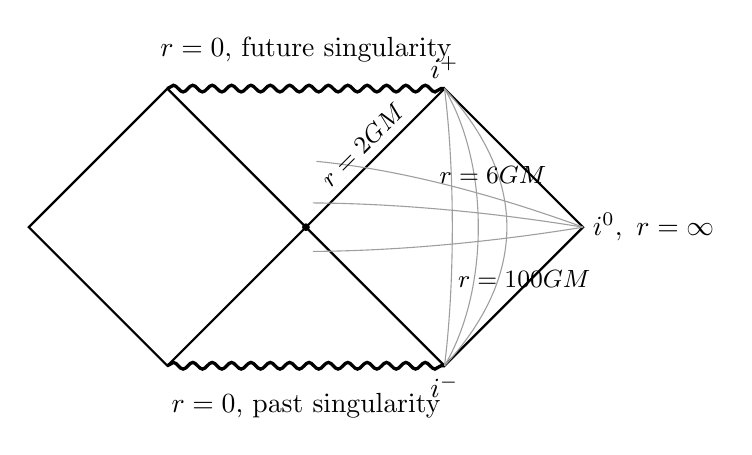
\begin{tikzpicture}[scale=0.88]
\coordinate (C) at (0,0);
\coordinate (TL) at (-2.0,2.0);
\coordinate (L) at (-4.0,0);
\coordinate (BL) at (-2.0,-2.0);
\coordinate (TR) at (2.0,2.0);
\coordinate (R) at (4.0,0);
\coordinate (BR) at (2.0,-2.0);
\draw[thick] (C)--(TL)--(L)--(BL)--(C);
\draw[thick] (C)--(TR)--(R)--(BR)--(C);
\draw[very thick,decorate,decoration={snake,amplitude=1.2pt,segment length=7pt}] (TL)--(TR);
\draw[very thick,decorate,decoration={snake,amplitude=1.2pt,segment length=7pt}] (BL)--(BR);
\draw[gray!75] (TR) .. controls (2.15,0.8) and (2.15,-0.8) .. (BR);
\draw[gray!75] (TR) .. controls (2.65,0.9) and (2.65,-0.9) .. (BR);
\draw[gray!75] (TR) .. controls (3.20,0.7) and (3.20,-0.7) .. (BR);
\draw[gray!75] (0.15,0.95) .. controls (1.5,0.82) and (2.9,0.40) .. (R);
\draw[gray!75] (0.10,0.35) .. controls (1.5,0.34) and (2.9,0.18) .. (R);
\draw[gray!75] (0.10,-0.35) .. controls (1.5,-0.34) and (2.9,-0.18) .. (R);
\fill (C) circle (1.6pt);
\node[above] at (TR) {\(i^+\)};
\node[below] at (BR) {\(i^-\)};
\node[right] at (R) {\(i^0,\ r=\infty\)};
\node[above] at (0,2.25) {\(r=0\), future singularity};
\node[below] at (0,-2.25) {\(r=0\), past singularity};
\node[rotate=45,above,font=\small] at (1.0,1.0) {\(r=2GM\)};
\node[font=\small] at (2.70,0.75) {\(r=6GM\)};
\node[font=\small] at (3.15,-0.75) {\(r=100GM\)};
\end{tikzpicture}
\caption{The right exterior resembles the flat wedge at large radius. Its inner null edge is \(r=2GM\) when \(c=1\); the other labeled radii are schematic examples.}
\label{fig:l05-eternal-schwarzschild}
\end{figure}

Far from the hole, the exterior looks increasingly like compactified flat space. Lines such as \(r=6GM\) and \(r=100GM\) approach the behavior of ordinary constant-radius worldlines. The inner boundary of the exterior is at
\begin{equation}
r=2GM
\end{equation}
in units \(c=1\).

Near the center, the comparison with flat space fails. A radial ray in Minkowski space reaches \(r=0\) and re-emerges on the opposite physical side. A future-directed ray inside Schwarzschild does not bounce. It ends on the spacelike singularity at \(r=0\). That causal difference is what the collapse construction must preserve.

\section{The Theorem That Lets Us Join the Pieces}

The missing ingredient first appears in Newtonian gravity. For a spherically symmetric mass distribution, Gauss's law gives
\begin{equation}
\oint\mathbf g\cdot d\mathbf A=-4\pi G M_{\mathrm{enc}},
\end{equation}
and therefore
\begin{equation}
\mathbf g(r)=-\frac{G M_{\mathrm{enc}}(r)}{r^2}\,\hat{\mathbf r}.
\label{eq:l05-shell-theorem}
\end{equation}
Matter outside the sphere of radius \(r\) contributes no net field there. For a hollow shell of total mass \(M\),
\begin{equation}
\mathbf g=
\begin{cases}
0, & r<R_{\mathrm{shell}},\\[3pt]
-\dfrac{GM}{r^2}\hat{\mathbf r}, & r>R_{\mathrm{shell}}.
\end{cases}
\end{equation}

Birkhoff's theorem is the relativistic replacement. Every spherically symmetric vacuum region is locally a Schwarzschild region with a constant mass parameter. The empty interior of a spherical shell has mass parameter zero and is locally Minkowski; the exterior has mass parameter \(M\) and is Schwarzschild:
\begin{equation}
\text{inside the shell: }M_{\mathrm{enc}}=0,
\qquad
\text{outside the shell: }M_{\mathrm{enc}}=M.
\label{eq:l05-birkhoff}
\end{equation}
The statement remains useful while the shell moves, because the vacuum regions on either side remain spherically symmetric.

\editorialnote{Flat inside is a local statement. A static shell can change the normalization of the interior time coordinate even though the interior curvature vanishes. For a moving or null shell, the two vacuum metrics must be matched across the shell; the idealized construction is a thin-shell junction, closely related to the ingoing Vaidya geometry. None of these qualifications changes the causal cut-and-paste argument used here.}

For a laboratory image, imagine a sphere densely covered with synchronized lasers, as at a large inertial-confinement facility, all fired inward at once. In the idealization there is no apparatus, only a perfectly spherical shell of light. The shell carries energy \(E\), so the exterior mass parameter is
\begin{equation}
M=\frac{E}{c^2},
\end{equation}
or simply \(E=M\) in natural units. Because the shell moves at light speed, it is an ingoing null line on the reduced diagram. Each point on that line represents a whole spherical wavefront, not one photon trajectory.

\section{Sewing the Collapse Spacetime}

Start with flat spacetime and draw the ingoing null shell. The region inside the shell is correct: Birkhoff's theorem says it is flat. The region outside is wrong, because the exterior must already know the shell's total mass through its Schwarzschild geometry.

Now draw the same shell in the eternal Schwarzschild diagram. There the region outside the shell is correct. The white hole, the second exterior, and the inappropriate part of the black-hole interior are wrong for a collapse beginning in ordinary empty space, so erase them.

\begin{figure}[htbp]
\centering

\includegraphics[width=0.72\textwidth]{lecture_05_figure_05.png}
\caption{The null shell, in red, drawn across the Schwarzschild diagram while the correct exterior portion is being isolated.}
\lectureframe{00:32:00.000}
\end{figure}

The shell reaches \(r=0\) in the flat piece. In the Schwarzschild piece it reaches the beginning of the future singularity. These are the same endpoint. Pasting the flat interior to the Schwarzschild exterior along the shell gives the simplest spacetime of black-hole formation.

\begin{classroomqa}
\audiencequestion{At the upper-left joining point, is the flat-space endpoint really the same as the point on the Schwarzschild side?\lecturetimestamp{00:34:50}}
\lecturerresponse{Yes. The flat-space shell shrinks to \(r=0\), and the Schwarzschild singularity is also at \(r=0\). The two points being identified have the same geometric meaning: the two-sphere has shrunk to zero size.}
\end{classroomqa}

\begin{figure}[htbp]
\centering
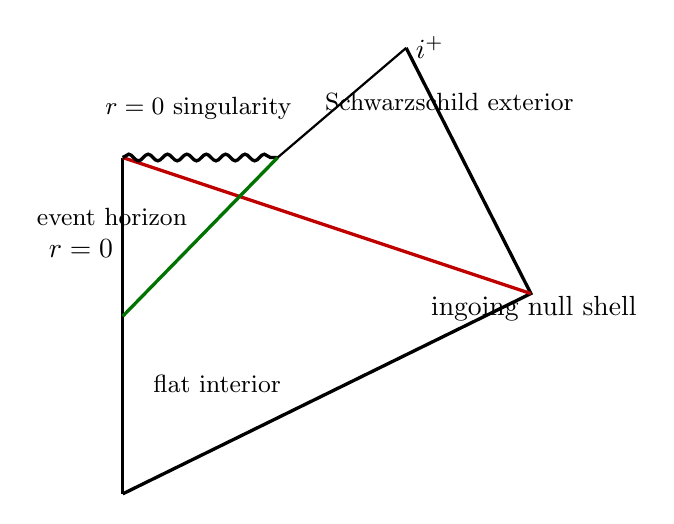
\begin{tikzpicture}[scale=0.96]
\coordinate (A) at (0,-2.8);
\coordinate (B) at (0,1.65);
\coordinate (C) at (2.05,1.65);
\coordinate (D) at (5.4,-0.15);
\coordinate (E) at (3.75,3.10);
\coordinate (H0) at (0,-0.45);
\draw[very thick] (A)--(B);
\draw[very thick] (A)--(D)--(E);
\draw[very thick,red!75!black] (D)--(B);
\draw[very thick,decorate,decoration={snake,amplitude=1.2pt,segment length=7pt}] (B)--(C);
\draw[very thick,green!45!black] (H0)--(C);
\draw[thick] (C)--(E);
\node[left] at (0,0.45) {\(r=0\)};
\node[below right] at (3.95,-0.05) {ingoing null shell};
\node[font=\small] at (1.25,-1.35) {flat interior};
\node[font=\small,anchor=west] at (2.55,2.38) {Schwarzschild exterior};
\node[above,font=\small] at (1.0,2.02) {\(r=0\) singularity};
\node[above left,font=\small] at (0.98,0.62) {event horizon};
\node[right] at (E) {\(i^+\)};
\end{tikzpicture}
\caption{The collapse geometry. The red shell joins a flat interior to a Schwarzschild exterior. The green event horizon begins earlier in the flat region and ends at the future boundary of the black-hole region.}
\label{fig:l05-collapse}
\end{figure}

This construction answers a question left by the eternal solution. A black hole made from collapse has no past white hole and no second asymptotic universe. It still has a future singularity.

\section{The Horizon Is a Global Boundary}

The old label \(r=2GM\) identified the horizon in the stationary Schwarzschild geometry, but it is not the definition needed in a dynamical spacetime.

\begin{definition}
The future event horizon is the boundary of the set of events that can send a future-directed causal signal to future null infinity.
\end{definition}

On the collapse diagram, trace the outgoing null ray that just fails to escape. Rays just outside it reach infinity; rays just inside it end at the singularity. That separator is the true horizon.

\begin{figure}[htbp]
\centering

\includegraphics[width=0.72\textwidth]{lecture_05_figure_06.png}
\caption{The completed board construction. The incoming shell is red and the event horizon is green; part of the green line lies in the still-flat region below the shell.}
\lectureframe{00:39:10.000}
\end{figure}

The startling feature is now unavoidable. The horizon extends backward into a region where the shell has not yet arrived. The geometry there is locally flat, and an observer crossing that line detects no curvature pulse, wall, or flash. Nevertheless, the observer is already unable to reach infinity, because the future shell will close every possible escape route. Event horizons are teleological in precisely this global sense: locating one requires knowledge of the spacetime's entire future.\editorialnote{No local experiment can determine that a smooth event horizon has just been crossed. Other notions, such as apparent or trapping horizons, are more local and need not coincide with the event horizon during collapse.}

The drain analogy isolates the causal idea. Imagine a rower near a plugged drain in a motionless lake. If the plug remained forever, the rower could leave. If someone is certain to pull it, the later current may make escape impossible even though no water is moving yet. A frozen Niagara Falls makes the same point: calm water does not guarantee a future route to safety.

\begin{classroomqa}
\audiencequestion{Is the plug pulled because the spherical shell of light becomes more and more concentrated?\lecturetimestamp{00:43:13}}
\lecturerresponse{The concentration creates the black hole, but the drain story is being used for a narrower purpose: one can already be beyond the point of no return before anything locally dramatic occurs.}
\end{classroomqa}

\subsection{A horizon made of growing spheres}

Every point on the reduced horizon represents an \(S^2\). At the horizon's first point that sphere has zero area. Moving upward along the horizon, the sphere grows until its areal radius reaches
\begin{equation}
R_s=\frac{2GM}{c^2}.
\end{equation}
It remains at that size for a stationary hole and grows again if more energy falls in.

\editorialnote{In the idealized spherical collapse diagram, the horizon generators meet at a formation point, or crease, on \(r=0\). It is this limiting two-sphere that has zero area; the statement should not be read as a finite Schwarzschild horizon suddenly shrinking to a point.}

\subsection{What the distant observer can reconstruct}

The long discussion that follows separates an observer already inside the global horizon from the history by which that observer came to be there.

\begin{classroomqa}
\audiencequestion{What is the status of the person trapped before the shell arrives? Is that person outside the horizon from the distant observer's point of view?\lecturetimestamp{00:44:03}}
\lecturerresponse{No. Once the worldline is behind the event horizon, its future reaches the singularity and no new signal from it reaches the distant observer. The person did not begin existence there, however. Earlier particles, ancestors, or other precursor energy entered from a region that was visible.}
\end{classroomqa}

The distant observer may therefore see the precursor matter approaching the horizon without ever receiving a signal from beyond it. There is no contradiction in seeing through the incoming shell: it is made of light, and the observer can also see the shell itself and infer that a black hole has formed.

\begin{classroomqa}
\audiencequestion{Does the line of sight pass through the collapsing shell, and can the outside observer still know that the hole formed?\lecturetimestamp{00:46:51}}
\lecturerresponse{Yes. The observer sees the incoming shell and can receive light whose path crosses it while that light is still able to escape. What looks strange is that the precursor matter approaches the newly determined horizon even before the shell reaches the center.}
\end{classroomqa}

\begin{classroomqa}
\audiencequestion{Does this continue the rule that, from outside, matter looks as though it has been compressed onto the horizon?\lecturetimestamp{00:47:49}}
\lecturerresponse{Yes. In the exterior description it remains associated with the horizon, becoming ever more redshifted, until the later quantum process of black-hole evaporation changes the story.}
\end{classroomqa}

This outside description motivates the next subject. If information appears plastered onto a two-dimensional surface, it is less surprising that black-hole entropy scales with that surface's area.

\section{Entropy and the Temperature Seen from Infinity}

Near a large horizon we may replace the spherical surface by a local plane, just as we use a flat-Earth approximation in a small laboratory. Two facts from the earlier discussion are then brought together:
\begin{equation}
S_{\mathrm{BH}}\propto A_H,
\qquad
\Delta A_H\sim \ell_P^2
\quad\hbox{per added bit, schematically}.
\end{equation}
The one-bit-per-Planck-area statement is a mnemonic for the area law, not a microscopic derivation.

The Hawking temperature measured far from a Schwarzschild black hole is
\begin{equation}
T_H=\frac{\hbar c^3}{8\pi GMk_B}.
\label{eq:l05-hawking}
\end{equation}
With \(R_s=2GM/c^2\),
\begin{equation}
T_H=\frac{\hbar c}{4\pi k_B R_s}.
\label{eq:l05-hawking-radius}
\end{equation}
Thus larger holes are colder.

\begin{classroomqa}
\audiencequestion{Can temperature depend on position?\lecturetimestamp{00:52:43}}
\lecturerresponse{In ordinary conversation it plainly can: New York and Stanford need not have the same temperature. The sharper question concerns a system in gravitational thermal equilibrium. There, local thermometer readings can vary with height even though the redshifted equilibrium temperature is constant.}
\end{classroomqa}

Temperature is read through local kinetic energies. In a dilute atmosphere above a heated Earth, molecules lose kinetic energy as they climb and gain it as they fall. Photons are redshifted upward and blueshifted downward. A low thermometer and a high thermometer therefore need not register the same local energy scale.

For a static spacetime, the equilibrium relation is
\begin{equation}
T_{\mathrm{loc}}(r)\sqrt{-g_{tt}(r)}=T_\infty,
\label{eq:l05-tolman}
\end{equation}
the Tolman law. The Hawking temperature in Equation~\eqref{eq:l05-hawking} is \(T_\infty\), the reading normalized at infinity.

\section{The Hot Static Atmosphere Near the Horizon}

Let \(\rho\) be proper distance outward from the horizon. Close to a large Schwarzschild horizon, Equation~\eqref{eq:l05-tolman} becomes
\begin{equation}
k_B T_{\mathrm{loc}}(\rho)
\simeq\frac{\hbar c}{2\pi\rho},
\label{eq:l05-local-temperature-si}
\end{equation}
or, in units \(c=\hbar=k_B=1\),
\begin{equation}
T_{\mathrm{loc}}(\rho)=\frac{1}{2\pi\rho}.
\label{eq:l05-local-temperature}
\end{equation}

\begin{figure}[htbp]
\centering

\includegraphics[width=0.72\textwidth]{lecture_05_figure_07.png}
\caption{The asymptotic Hawking temperature and the near-horizon local temperature \(T(\rho)=1/(2\pi\rho)\) on the board.}
\lectureframe{01:02:40.000}
\end{figure}

A tiny thermometer held on a cable at fixed \(\rho\) reports an increasing temperature as it is lowered. An atom maintained in that static atmosphere becomes excited, then ionized, then dissociated; at still larger local energies even nuclei and hadrons cease to remain intact. Lowering a person feet first gives the memorable diagnosis: a hot foot.

The word \emph{held} is essential. The divergent temperature belongs to a stationary, accelerated detector and to the redshifted thermal atmosphere defined relative to the exterior time. A freely falling detector follows a different trajectory. For a sufficiently large hole in a regular quantum state, it need not encounter a divergent bath at the horizon.\editorialnote{This distinction separates the Tolman/acceleration temperature of static observers from the regular local experience of a freely falling observer. The lecture deliberately turns that contrast into an operational puzzle rather than resolving it by terminology alone.}

The ionization threshold makes the conflict concrete.

\begin{classroomqa}
\audiencequestion{How much energy is required to ionize hydrogen?\lecturetimestamp{01:06:53}}
\lecturerresponse{The class gives \(13\) electron volts, correctly identifying the \(13.6\,\mathrm{eV}\) ground-state ionization energy. The accompanying estimate of a few thousand kelvin is too small, but only the existence of a finite threshold is needed for the argument.}
\end{classroomqa}

Indeed,
\begin{equation}
\frac{13.6\,\mathrm{eV}}{k_B}\simeq1.58\times10^5\,\mathrm{K}.
\end{equation}
There is therefore some small proper distance \(\rho_{\mathrm{ion}}\) at which the static temperature reaches the ionization scale. A static extrapolation says the atom should already be ionized there, outside the horizon. A freely falling atom, by contrast, expects no local wall and can cross the horizon in finite proper time. Can an outside observer perform an experiment that decides between these descriptions?

\section{A Heisenberg Microscope}

Before applying the question to a black hole, recall the photon microscope. To locate a particle with resolution \(\Delta x\), the probe wavelength must obey
\begin{equation}
\lambda\lesssim\Delta x.
\end{equation}
One photon then carries momentum of at least
\begin{equation}
p_\gamma\gtrsim\frac{\hbar}{\Delta x}.
\label{eq:l05-microscope}
\end{equation}
Scattering that photon creates a recoil of the same order. If one first measures position and immediately checks velocity, the second measurement sees a state changed by the first. The experiment creates the condition it was intended to exclude.

\begin{figure}[htbp]
\centering

\includegraphics[width=0.70\textwidth]{lecture_05_figure_08.png}
\caption{The microscope estimates \(\Delta x\gtrsim\lambda\) and \(p_\gamma\gtrsim\hbar/\Delta x\).}
\lectureframe{01:11:50.000}
\end{figure}

This is not merely a limitation of classical optics. Classical waves could be made arbitrarily weak; quantum mechanics requires at least one quantum in a successful detection event. Improving the spatial resolution therefore forces a finite momentum transfer.

\section{The Near-Horizon Experiment}

Now let an atom fall through the layer beginning at \(\rho_{\mathrm{ion}}\). Relative to the static frame it is moving inward at nearly \(c\), so the available interval before horizon crossing is of order
\begin{equation}
\Delta\tau\sim\frac{\rho_{\mathrm{ion}}}{c}.
\label{eq:l05-fall-time}
\end{equation}
After crossing, no result can be sent back to the exterior. The measurement must distinguish an intact atom from an ionized one during this short interval.

Resolving the atom within the layer requires
\begin{equation}
\lambda\lesssim\rho_{\mathrm{ion}}.
\end{equation}
The probe energy is consequently bounded by
\begin{equation}
E_\gamma=cp_\gamma
\gtrsim\frac{\hbar c}{\rho_{\mathrm{ion}}}.
\label{eq:l05-probe-energy}
\end{equation}
Apart from the factor \(2\pi\), this is the same scale as Equation~\eqref{eq:l05-local-temperature-si}:
\begin{equation}
E_\gamma\gtrsim2\pi k_B T_{\mathrm{loc}}(\rho_{\mathrm{ion}}).
\label{eq:l05-probe-temperature}
\end{equation}
The photon energetic enough to resolve the event is also energetic enough to ionize the atom.

\begin{figure}[htbp]
\centering

\includegraphics[width=0.72\textwidth]{lecture_05_figure_09.png}
\caption{The near-horizon estimate on the board: \(\lambda<\rho\) forces a local probe energy of order \(\hbar c/\rho\).}
\lectureframe{01:18:30.000}
\end{figure}

\begin{classroomqa}
\audiencequestion{Would that high-energy photon ionize the atom even in its freely falling frame?\lecturetimestamp{01:19:07}}
\lecturerresponse{Yes. The atom is struck by a real energetic quantum and recoils or ionizes in its own local frame. The measurement does not reveal an undisturbed fall; it replaces it with a disturbed one.}
\end{classroomqa}

\begin{classroomqa}
\audiencequestion{What if the atom simply falls and no one performs the experiment?\lecturetimestamp{01:19:39}}
\lecturerresponse{Then this particular disturbance is absent. If an outside observer does perform the high-resolution experiment, the atom is in trouble. The argument concerns what can be verified from outside, not a proof that an unmeasured infaller burns.}
\end{classroomqa}

\subsection{Can a thermometer or transmitter do better?}

Moving the apparatus does not remove the information problem.

\begin{classroomqa}
\audiencequestion{Could one measure farther away, infer the gradient, or let a freely falling thermometer record the temperature and recover it later?\lecturetimestamp{01:19:51}}
\lecturerresponse{To learn the near-horizon record, something must interact with the thermometer and return information in quanta. Turning the thermometer around requires violent acceleration, while reading it remotely requires emission or scattering. Either route changes the physical system whose undisturbed history was to be tested.}
\end{classroomqa}

\begin{classroomqa}
\audiencequestion{Is the high probe energy needed for small resolution the same difficulty as getting the reflected observation away from the near-horizon region?\lecturetimestamp{01:21:51}}
\lecturerresponse{They are two sides of the same redshifted scale. The photon can be low in energy when it finally reaches infinity because it loses energy climbing out, but it must have high local frequency where it resolves the atom.}
\end{classroomqa}

\editorialnote{A photon emitted just outside the horizon need not possess a large energy merely to escape. The decisive requirement here is that it encode the event within a proper time and distance of order \(\rho\); gravitational redshift then relates that large local frequency to a much smaller asymptotic one.}

\begin{classroomqa}
\audiencequestion{Could the object emit the information itself rather than being struck by an external photon?\lecturetimestamp{01:22:51}}
\lecturerresponse{Yes, but the local emission still needs the bandwidth required to identify what happened during the short interval. Emission also gives the object recoil. Replacing reflected light by a transmitter does not produce a cost-free record.}
\end{classroomqa}

\begin{classroomqa}
\audiencequestion{The falling atom has a preferred direction. Is its directed kinetic energy being called temperature?\lecturetimestamp{01:23:10}}
\lecturerresponse{No. Throwing a baseball does not make the baseball hot. Bulk infall energy and thermal agitation are distinct. The temperature in the argument belongs to the surrounding static radiation atmosphere, not to the center-of-mass motion of the atom.}
\end{classroomqa}

\begin{classroomqa}
\audiencequestion{Could a co-falling laboratory use a magnetic field to test whether the atom is ionized?\lecturetimestamp{01:23:50}}
\lecturerresponse{A laboratory can perform a local test. The difficulty is communicating its result back outside before crossing. That communication again requires an interaction and outgoing quanta with the necessary local resolution.}
\end{classroomqa}

\begin{classroomqa}
\audiencequestion{Would a transmitter built into the thermometer need so much local energy that it destroys the apparatus?\lecturetimestamp{01:24:57}}
\lecturerresponse{That is the same obstruction in engineering form. Near enough to the horizon, the signal energy required on the relevant local scale is comparable to the thermal scale being tested.}
\end{classroomqa}

\begin{classroomqa}
\audiencequestion{Is the high-temperature region so thin that there is no time to carry out the measurement leisurely?\lecturetimestamp{01:25:15}}
\lecturerresponse{Exactly. Its proper thickness is of order \(\rho\), and the crossing time is of order \(\rho/c\). One may describe the limitation as spatial resolution or temporal bandwidth; either description demands high local momentum or energy.}
\end{classroomqa}

The corresponding time-bandwidth estimate is
\begin{equation}
\Delta E\,\Delta\tau\gtrsim\hbar.
\end{equation}
Here this should be read as a Fourier or operational resolution bound, not as an operator uncertainty relation identical in status to \(\Delta x\,\Delta p\geq\hbar/2\). The lecture invokes time-energy uncertainty heuristically; Equation~\eqref{eq:l05-probe-energy}, derived from spatial resolution, is the firmer part of the argument.

\begin{classroomqa}
\audiencequestion{Could one use lower-energy, lower-resolution probes on many atoms and recover the answer statistically?\lecturetimestamp{01:26:26}}
\lecturerresponse{This is a sensible question, and it is left open in the classroom. Each atom provides only one passage, and any recovered signal must still carry enough information to identify the short near-horizon event. The lecture appeals to the uncertainty principle but does not supply a complete statistical no-go proof.}
\end{classroomqa}

\enlargethispage{2\baselineskip}
\section{What Has and Has Not Been Established}

The argument does not predict that a freely falling person must feel the divergent static temperature.

\begin{classroomqa}
\audiencequestion{Are we saying that we can predict the falling person will not feel the temperature?\lecturetimestamp{01:27:38}}
\lecturerresponse{No. The result is narrower: an exterior experiment designed to confirm that the atom did not experience the high-temperature disturbance creates a disturbance of the same scale. That is all this operational analysis establishes.}
\end{classroomqa}

Thus the conclusion is not a firewall theorem, nor a proof that the infaller is burned, nor a proof that nothing happens. It is a limit on exterior verification: \emph{resolving the undisturbed near-horizon event requires a probe that disturbs it}.
If the experiment is performed, its quanta produce the effect it was meant to test. If it is not performed, this argument alone assigns no additional experimentally accessible fact. The comparison with the two-slit experiment is deliberate: asking which slit was taken without a path measurement and asking what an exterior apparatus certifies without an interaction are both attempts to attach an operational answer where the proposed evidence cannot be obtained.
